\documentclass[journal]{new-aiaa}
%\documentclass[conf]{new-aiaa} for conference papers
\usepackage[utf8]{inputenc}
\usepackage{textcomp}

\usepackage{graphicx}
\usepackage{amsmath}
\usepackage[version=4]{mhchem}
\usepackage{siunitx}
\usepackage{longtable,tabularx}
\graphicspath{ {/Users/mattwilliams/Documents/GitHubClonedRepos/PythonCFD/uCFD/Project1_files} }
\setlength\LTleft{0pt} 

\title{CFD Analysis of Cavity Driven Flow with Heat Transfer}

\author{LCDR Matt Williams \footnote{matt.williams@alum.mit.edu}}
\affil{Course Director, US Navy Engineering Duty Officer School, Port Hueneme, CA}

\begin{document}
\maketitle
\begin{abstract}
This is the heated driven cavity project, assigned to students during CHEN 6355 (uCFD) by Tony Saad at the University of Utah. The physical problem is a Cartesian cavity with lid-driven flow, subject to uniform heating at one surface, and adiabatic conditions on all others. The numerical equations to be solved will be the vorticity-streamfunction formulation of the Navier-Stokes momentum equations, along with the energy equation. A body-force gravitational term will be added to the momentum equations, with the only active component being the acceleration due to gravity in the y-direction.
\end{abstract}

\section{Problem Description}
\begin{figure}[hbt!]
\centering
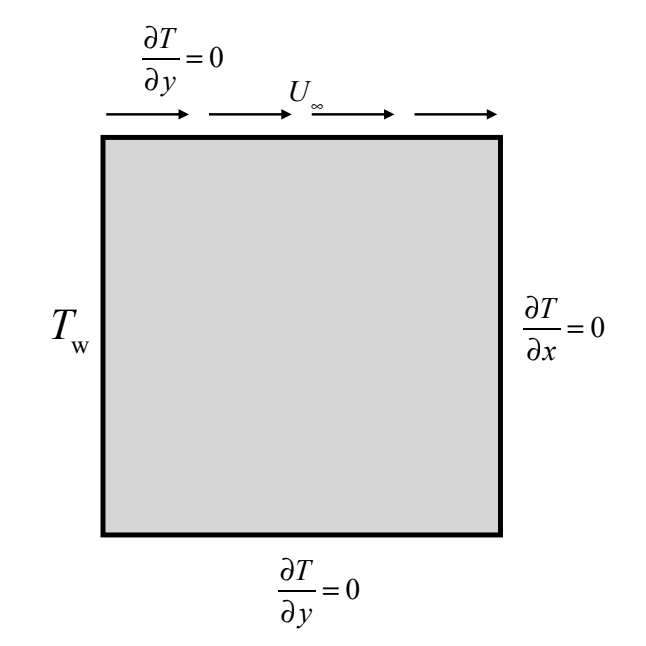
\includegraphics[width=.5\textwidth]{cavity}
\caption{Heated cavity with lid-driven flow}
\label{fig:domain} 
\end{figure}

The physical domain is shown in Figure \ref{fig:domain}. The boundaries are rigid and non-porous. The left wall is subject to a uniform temperature, and the top boundary is subjected to a uniform velocity. The top, bottom, and right boundaries are adiabatic. That is, $\frac{\partial T}{\partial x_i} = 0$ on the boundary. The fluid inside the domain is considered incompressible, therefore:

\begin{equation}
\label{equation:incompressible}
\frac{D\rho }{Dt} =\frac{\partial \rho }{\partial t} +\textbf{u}\cdot \nabla \rho =0
\end{equation}

From the properties of the divergence operator, we have
\begin{equation}
\label{equation:divergence}
\nabla \cdot (\rho \textbf{u})\  =\ \textbf{u}\cdot \nabla \rho \  +\  \rho \nabla \cdot \textbf{u}
\end{equation}


\begin{equation}
\label{equation:divergence2}
\nabla \cdot (\rho \textbf{u})- \rho \nabla \cdot \textbf{u}\  =\ \textbf{u}\cdot \nabla \rho 
\end{equation}

Substituting the result in Equation \ref{equation:divergence2} into Equation \ref{equation:incompressible} gives

\begin{equation}
\label{equation:incompressible2}
\frac{D\rho }{Dt} =\frac{\partial \rho }{\partial t} +\nabla \cdot (\rho \textbf{u})-\rho \nabla \cdot \textbf{u}=0
\end{equation}

The first two terms on the right-hand side are the continuity equation and are identically zero, therefore the incompressibility condition leaves

\begin{equation}
\label{equation:incompressible3}
\nabla \cdot \textbf{u}=0
\end{equation}

Which states that for incompressible flows, the divergence of the velocity is zero. This result is also obtained by the non-conservative form of following a fluid parcel that is subject to a changing shape, where a small column of fluid has height $\textbf{V}\cdot \textbf{n}\Delta t$ and volume $\Delta V = \textbf{V}\cdot \textbf{n}\Delta t dS$, which can be rewritten as $\Delta V = \textbf{V}\cdot \Delta t \textbf{dS}$. Therefore, the entire fluid volume is the sum over the entire surface. In the limit as $dS\rightarrow 0$, the equation becomes $dV\  =\  \int \int_{S} \textbf{V}\cdot \bigtriangleup t\textbf{dS}$. Dividing by $\Delta t$ in the limit, and applying the divergence theorem, we have:

\begin{equation}
\label{equation:incompressible4}
\frac{DV}{Dt} \  =\  \iiint_{V} (\nabla \cdot \textbf{V})dV
\end{equation}

where the substantial derivative has been used because we are following a fluid parcel. Now, if the fluid volume size is reduced, then the integration over the volume becomes equal to the integrand itself:

\begin{equation}
\label{equation:incompressible5}
\frac{D(\delta V)}{Dt} \  = (\nabla \cdot \textbf{V})\delta V
\end{equation}

Dividing by $\delta V$:

\begin{equation}
\label{equation:incompressible6}
\frac{1}{\delta V}\frac{D(\delta V)}{Dt} \  = \nabla \cdot \textbf{V}
\end{equation}

In an incompressible flow, the fluid volume does not change, although the volume's shape may change. Therefore, Equation \ref{equation:incompressible6} is equal to zero, which again gives the result that the divergence of the velocity is zero for an incompressible flow.

The incompressible flow assumption leads to some simplifications of the Navier-Stokes equations. For this paper, "Navier-Stokes" equations refers explicitly to the momentum equations. Often, the continuity and energy equations are included in the terminology, but those will be referred to by name and are not included in the term "Navier-Stokes equations." The vector form of the Navier-Stokes equations is:

\begin{equation}
\label{equation:nsvec}
\frac{\partial \rho \textbf{u}}{\partial t} =-\nabla \cdot (\textbf{u}\rho \textbf{u})-\nabla p+\rho \textbf{f} + \mu \nabla^2 \textbf{u}
\end{equation}

where $\textbf{f}$ is a body force. We will include the Bousinessq approximation as the body force, which is given by $\beta(T-T_0)\textbf{g}$. This will provide coupling to the energy equation and account for gravitational effects and heating effects on the fluid.

We want to take this form of the Navier-Stokes equation and get the vorticity-streamfunction formulation. This is done by taking the curl of the equations:

\begin{equation}
\label{equation:nscurl}
\nabla \times \frac{\partial \rho \textbf{u}}{\partial t} =-\nabla \times \nabla \cdot (\textbf{u}\rho \textbf{u})-\nabla \times \nabla p+\nabla \times \rho \textbf{f}+ \nabla \times \nu \nabla^2 \textbf{u}
\end{equation}

Here, we have maintained the equation in conservative form. The divergence of the dyadic product of the velocity can be expanded:

\begin{equation}
\label{equation:dyadexpand}
\nabla \cdot (\vec{u} \vec{u} )\  =\  \vec{u} \cdot (\nabla \vec{u} )\  +(\nabla \cdot \vec{u} )\vec{u} 
\end{equation}

For incompressible flow, the second term on the right of Equation \ref{equation:dyadexpand} is zero. The first term on the right can be expanded as:

\begin{equation}
\label{equation:dotdyad}\
\vec{u} \cdot (\nabla \vec{u} )=\frac{1}{2} \nabla (\vec{u} \cdot \vec{u} )\  -\  \vec{u} \times (\nabla \times \vec{u} )
\end{equation}

Taking the cross product of Equation \ref{equation:dotdyad} gives:
\begin{equation}
\label{equation:cross}
\nabla \times \vec{u} \cdot (\nabla \vec{u} )=\nabla \times \nabla \frac{\left| \vec{u}^{2} \right|  }{2} \  -\  \nabla \times \vec{u} \times \vec{\omega } 
\end{equation}

The first term on the right of Equation \ref{equation:cross} is identically zero by the identities of vector calculus. The last term on the right can be expanded to:

\begin{equation}
\label{equation:cross2}
\nabla \times \vec{u} \times \vec{\omega } =(\vec{u} \cdot \nabla )\vec{\omega } -(\vec{\omega } \cdot \nabla )\vec{u} +\vec{\omega } (\nabla \cdot \vec{u} )+\vec{u} (\nabla \cdot \vec{\omega } )
\end{equation}

The last two terms on the right of Equation \ref{equation:cross2} are zero. Therefore, finally:
\begin{equation}
\label{equation:cross3}
\nabla \times \vec{u} \cdot (\nabla \vec{u} )=(\vec{\omega } \cdot \nabla )\vec{u} -(u\cdot \nabla )\vec{\omega } 
\end{equation}

Therefore, the curl of Equation \ref{equation:nsvec} is:

\begin{equation}
\label{equation:vorticity}
\frac{\partial \omega }{\partial t} +\vec{u} \cdot (\nabla \vec{\omega } )-(\vec{\omega } \cdot \nabla )\vec{u} =\nu \nabla^{2} \vec{\omega } +\nabla \times \vec{f} 
\end{equation}

Since this is a two-dimensional problem, there is no $\hat{k}$ component of $\vec{u}$,  and so the second term on the right is zero. The dyadic product of the gradient and the vorticity will still provide non-zero components:

\begin{equation}
\label{equation:dyad}
\nabla \vec{\omega } =\left[ \frac{\partial \omega }{\partial x} ik\  \frac{\partial \omega }{\partial y} jk\right]  
\end{equation}

We must analyze the curl of the Bousinnesq approximation. The only component that will vary with position is the temperature. Therefore, the resulting curl is $\beta*9.81*\frac{\partial T}{\partial x}\hat{k}$

Finally, the equation that is to be solved numerically is:

\begin{equation}
\label{equation:main}
\frac{\partial \omega }{\partial t} +\frac{\partial \psi }{\partial x} \frac{\partial \omega }{\partial y} -\frac{\partial \psi }{\partial y} \frac{\partial \omega }{\partial x} =\nu \nabla^{2} \omega +\beta \ast 9.81\frac{\partial T}{\partial x} 
\end{equation}

where we have used the streamfunction identity $u=-\frac{\partial \psi}{\partial y}$ and $v=\frac{\partial \psi}{\partial x}$. The quantity that is desired from the solution is the vorticity. We can couple to vorticity and the streamfunction from the definition of the vorticity:

\begin{equation}
\label{equation:vorticity}
\frac{\partial^{2} \psi }{\partial x^{2}} +\frac{\partial^{2} \psi }{\partial y^{2}} =-\omega 
\end{equation}

Finally, we need a way to couple the temperature, which will be via the energy equation:

\begin{equation}
\label{equation:energy}
\frac{\partial T}{\partial t} =-\nabla \cdot \vec{u} T+\frac{k}{\rho c_{p}} \nabla^{2} T
\end{equation}

The velocity must be rewritten in terms of the streamfunction, which will reformulate Equation \ref{equation:energy} to be:

\begin{equation}
\label{equation:energy1}
\frac{\partial T}{\partial t} =-\left( \frac{\partial uT}{\partial x} +\frac{\partial vT}{\partial y} \right)  +\frac{k}{\rho c_{p}} \nabla^{2} T
\end{equation}

The partial derivative terms in Equation \ref{equation:energy1} must be expanded in order to re-write the velocity in terms of the streamfunction:

\begin{equation}
\label{equation:energy2}
\frac{\partial T}{\partial t} =-\left( u\frac{\partial T}{\partial x} +T\frac{\partial u}{\partial x} +v\frac{\partial T}{\partial y} +T\frac{\partial v}{\partial y} \right)  +\frac{k}{\rho c_{p}} \nabla^{2} T
\end{equation}

The terms multiplied by $T$ will cancel out when written in terms of the streamfunction, as the partial derivatives will result in mixed derivatives of the same quantity. Writing the velocity in terms of the streamfunction gives the final form for the energy equation:

\begin{equation}
\label{equation:energyfinal}
\frac{\partial T}{\partial t} =-\left( -\frac{\partial \psi }{\partial y} \frac{\partial T}{\partial x} +\frac{\partial \psi }{\partial x} \frac{\partial T}{\partial y} \right)  +\frac{k}{\rho c_{p}} \nabla^{2} T
\end{equation}

The three equations that comprise our system to be solved are Equations \ref{equation:main}, \ref{equation:vorticity}, and \ref{equation:energyfinal}.

\section{Discretizing the Equations}
We must now take on the task of discretizing the equations to be solved in the previous section. We will use forward differences in time and centered differences in space, referred to as the FTCS scheme. 

We will begin by first discretizing the poisson streamfunction equation. If we include an over-relaxation term $\beta_r$, the discretization is
\begin{equation}
\label{equation:psidiscrete}
\psi^{k+1}_{ij} =\beta_{r} \frac{\Delta x^{2}\Delta y^{2}}{2\left( \Delta x^{2}+\Delta y^{2}\right)  } \omega^{n}_{ij} +\beta_{r} \frac{\Delta y^{2}}{2\left( \Delta x^{2}+\Delta y^{2}\right)  } \left( \psi^{k}_{i+1,j} +\psi^{k+1}_{i-1,j} \right)  +\beta_{r} \frac{\Delta x^{2}}{2\left( \Delta x^{2}+\Delta y^{2}\right)  } \left( \psi^{k}_{i,j+1} +\psi^{k+1}_{i,j-1} \right)  +(1-\beta_{r} )\psi^{k}_{ij} 
\end{equation}

This in an implicit scheme for $\psi^{k+1}_{ij}$. The streamfunction is not given in terms of time, but this equation will be iterated over in a subroutine until a defined level of convergence is reached prior to passing the solution to the main loop. The discretization of the vorticity transport equation is:

\begin{equation}
\begin{aligned}
\label{equation:omegadiscrete}
\omega^{n+1}_{ij} =\omega^{n}_{ij} +\Delta t\frac{\psi^{n}_{i+1,j} -\psi^{n}_{i-1,j} }{2\Delta x} \frac{\omega^{n}_{i,j+1} -\omega^{n}_{i,j-1} }{2\Delta y} -\Delta t\frac{\psi^{n}_{i,j+1} -\psi^{n}_{i,j-1} }{2\Delta y} \frac{\omega^{n}_{i+1,j} \omega^{n}_{i-1,j} }{2\Delta x} + \\ \
\Delta t\nu \left( \frac{\omega^{n}_{i+1,j} -2\omega^{n}_{ij} +\omega^{n}_{i-1,j} }{\Delta x^{2}} +\frac{\omega^{n}_{i,j+1} -2\omega^{n}_{ij} +\omega^{n}_{i,j-1} }{\Delta y^{2}} \right)  -\Delta t\beta g\frac{T^{n}_{i+1,j}-T^{n}_{i-1,j}}{2\Delta x} 
\end{aligned}
\end{equation}

The discretization of the energy equation is:

\begin{equation}
\begin{aligned}
\label{equation:omegadiscrete}
T^{n+1}_{ij}=T^n_{ij}+\Delta t\frac{\psi^{k}_{i,j+1} -\psi^{k}_{i,j-1} }{2\Delta y} \frac{T^{n}_{i+1,j}-T^{n}_{i-1,j}}{2\Delta x} +\Delta t \frac{\psi^{k}_{i+1,j} -\psi^{k}_{i-1,j} }{2\Delta x} \frac{T^{n}_{i,j+1}-T^{n}_{i,j-1}}{2\Delta y} +\Delta t\frac{k}{\rho c_{p}} \left(\frac{T^{n}_{i+1,j}-2T^{n}_{ij}+T^{n}_{i-1,j}}{\Delta x^{2}} +\frac{T^{n}_{i,j+1}-2T^{n}_{ij}+T^{n}_{i,j-1}}{\Delta y^{2}} \right)
\end{aligned}
\end{equation}

\section{Algorithm}
The order of operations for the solution algorithm will be:
\begin{itemize}
\item Compute $\omega^{n+1}_{ij}$ using the initial conditions for $\psi$ and $T$.
\item Compute the new temperature profile $T^{n+1}_{ij}$.
\item Update $\psi$
\item Repeat for desired number of iterations
\end{itemize}


\end{document}
